%!TEX root = bachelor.tex
\chapter{Methodik}
\label{ch:method}


\section{Kalibrierungsmuster}
\label{s:calibrationPattern}

\begin{figure}[!htb]
	\centering
	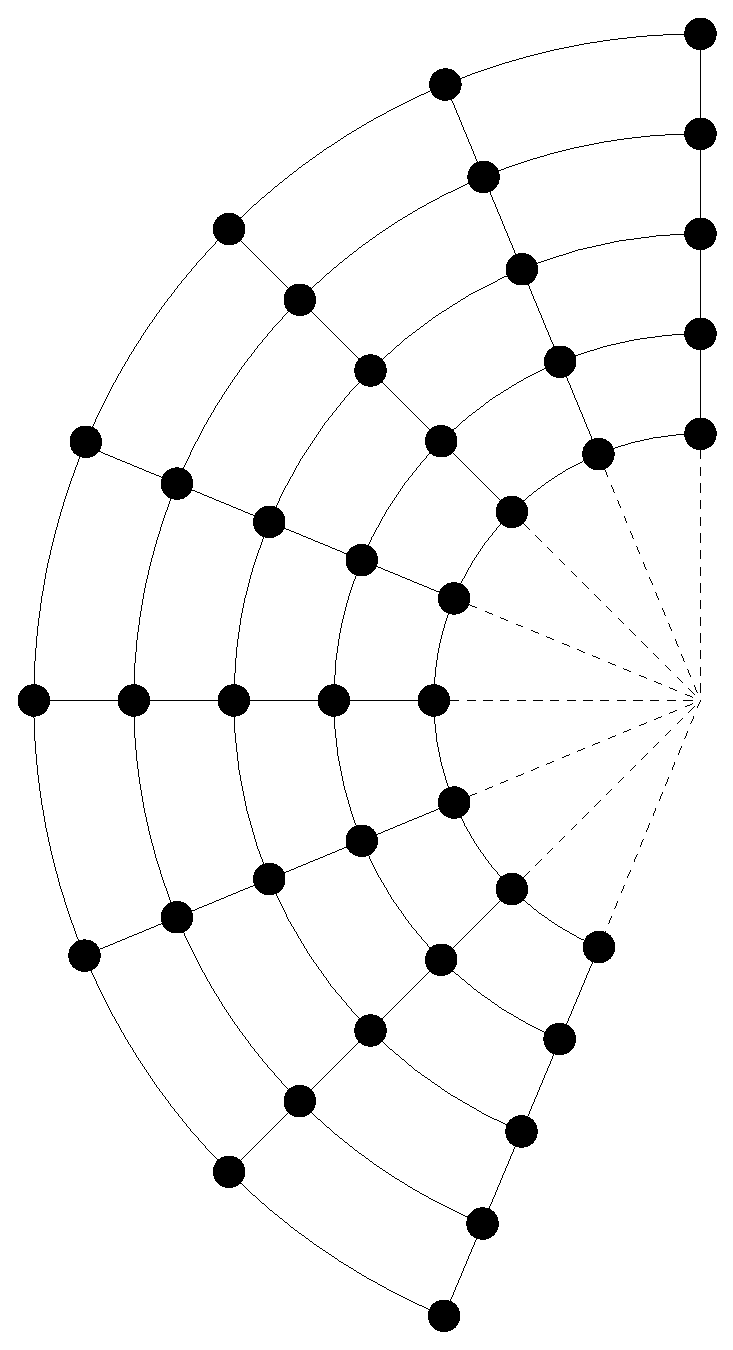
\includegraphics[scale=.4]{images/calibrationPattern.eps}
	\caption{Kalibrierungsmuster mit $n = 5, m = 7$}
	\label{fig:calibrationPattern}
\end{figure}
